\chapterfont{\color{DarkOrange}}  % sets colour of chapter
\sectionfont{\color{DarkOrange}}  % sets colour of sections
\subsectionfont{\color{DarkOrange}}  % sets colour of subsections

\renewcommand\pcolor{DarkOrange}
\renewcommand{\headrule}{\hbox to\headwidth{%
		\color{DarkOrange}\leaders\hrule height \headrulewidth\hfill}} % color of title
\fancyfoot[LE,RO]{\thepage}

{ \Large \leftwatermark{
		\put(-67,-66.5){ 1 }
		\put(-67,-91.5){ 2 }
		\put(-67,-116.5){ 3 }
		\put(-67,-141.5){ 4 }
		\put(-76.5,-176){
\includegraphics[scale=0.8]{img/thumbindex/thumbindex_DarkOrange.eps}} 
		\put(-67,-166.5){{\color{white} 5 }}
		\put(-67,-191.5){ 6 }
	} \rightwatermark{
		\put(350.5,-66.5){ 1 }
		\put(350.5,-91.5){ 2 }
		\put(350.5,-116.5){ 3 }
		\put(350.5,-141.5){ 4 }
		\put(350.5,-176){
\includegraphics[scale=0.8]{img/thumbindex/thumbindex_DarkOrange.eps}} 
		\put(350.5,-166.5){ {\color{white} 5 } }
		\put(350.5,-191.5){ 6 }
}}

\chapter[Brain expression quantitative trait locus and network analysis reveals downstream effects and putative drivers for neurological diseases ]{Brain expression quantitative trait locus and network analysis reveals downstream effects and putative drivers for neurological diseases}
\chaptermark{}

\label{chap:chapter5-brain}

\noindent
\\
\\

Niek de Klein\textsuperscript{1,4,5,6}, Ellen A. Tsai\textsuperscript{2,6}, Martijn Vochteloo\textsuperscript{1,3,7}, Denis Baird\textsuperscript{2,7}, Yunfeng Huang\textsuperscript{2}, Chia-Yen Chen\textsuperscript{2}, Sipko van Dam\textsuperscript{1}, Omar El Garwany\textsuperscript{1,5}, Maria Zavodszky\textsuperscript{2}, Heiko Runz\textsuperscript{2,8}, Lude Franke\textsuperscript{1,4,8}, Harm-Jan Westra\textsuperscript{1,4,8}






\noindent
1. Department of Genetics, University Medical Center Groningen, University of Groningen, Hanzeplein 1, Groningen, The Netherlands \\
2. \emph{trans}lational Biology, Research \& Development, Biogen Inc., 225 Broadway, Cambridge, MA, USA \\
3. Institute for Life Science \& Technology, Hanze University of Applied Sciences, Zernikeplein 11, 9747 AS Groningen, The Netherlands \\
4. Oncode Investigator \\
5. Wellcome Sanger Institute, Wellcome Genome Campus, Hinxton, UK \\
6. These authors contributed equally \\
7. These authors contributed equally \\
8. These authors jointly supervised the work 
\\
\\

\newpage

\section*{Abstract}
Gaining insight into the downstream consequences of non-coding variants is an essential step towards the identification of therapeutic targets from genome-wide association study (GWAS) findings.  Here we have harmonized and integrated 8,727 RNA-seq samples with accompanying genotype data from multiple brain-regions from 14 datasets. This sample size enabled us to perform both \emph{cis}- and \emph{trans}-expression quantitative locus (eQTL) mapping. Upon comparing the brain cortex \emph{cis}-eQTLs (for 12,307 unique genes at FDR $<$ 0.05) with a large blood \emph{cis}-eQTL analysis (n=31,684 samples), we observed that brain eQTLs are more tissue specific than previously assumed. 

We inferred the brain cell type for 1,515 \emph{cis}-eQTLs by using cell type proportion information. We conducted Mendelian Randomization on 23 neurological traits using the \emph{cis}-eQTLs and found 159 significant findings that also passed colocalization. Of the 20 Multiple Sclerosis (MS) MR findings, three genes did not have a significant eQTL in blood tissue, underscoring the importance of building and using tissue-specific resources. Furthermore, two MS findings had cell-type specific signals, a neuron-specific \emph{cis}-eQTL for CYP24A1 and a macrophage specific \emph{cis}-eQTL for CLECL1.  

To further interpret GWAS hits, we performed \emph{trans}-eQTL analysis. We identified 2,589 \emph{trans}-eQTLs (at FDR $<$ 0.05) for 373 unique SNPs, affecting 1,263 unique genes, and 21 replicated significantly using single-nucleus RNA-seq data from excitatory neurons.  

We also generated a brain-specific gene-coregulation network that we used to predict which genes have brain-specific functions, and to perform a novel network analysis of MS, Alzheimer’s disease, Parkinson’s disease and amyotrophic lateral sclerosis GWAS data. This resulted in the identification of distinct sets of genes that show significantly enriched co-regulation with genes inside the associated GWAS loci, and which might reflect drivers of these diseases. 

All eQTL summary statistics and the brain specific co-regulation network are publicly available at \url{www.metabrain.nl}. 

\section{Introduction}
Brain-related traits, such as psychiatric and neurodegenerative diseases continue to be a massive global health burden: the World Health Organization estimates that 329 million individuals were affected by psychiatric diseases depression, bipolar disorder, and schizophrenia in 2017\cite{jamesGlobalRegionalNational2018}. Likewise, while 50 million people are living with dementia today, this is expected to rise to 152 million by 2050\cite{WorldAlzheimerReport2018}, with similar trajectories for other neurodegenerative diseases. While substantial progress has been made in uncovering the genetic basis of psychiatric and neurodegenerative diseases through genome-wide association studies (GWAS), much of how the identified genetic variants impact brain function is still unknown.

To translate from genetic signals to mechanisms, associations with gene expression levels, or expression quantitative trait loci (eQTL) have shown great potential. eQTLs can be divided in direct effects of local genetic variants (\emph{cis}-eQTLs) and indirect effects of distal variants (\emph{trans}-eQTLs). \emph{Cis}-eQTLs and \emph{trans}-eQTLs can aid interpretation of GWAS loci in several ways. Cis-eQTLs aid interpretation by identifying direct links between genes and phenotypes through causal inference approaches such as Mendelian randomization (MR) instrumented on QTLs and genetic colocalization analysis, whereas trans-eQTLs expose sets of downstream genes and pathways on which the effects of disease variants converge.  

eQTLs are dynamic features and vary with tissue, cell-type and additional factors such as response to stimulation. For an optimal interrogation of GWAS loci, it is therefore desirable to perform eQTL analyses in disease-relevant tissues\cite{donovanCellularDeconvolutionGTEx2020}. To help interpret GWAS of neurodegenerative and psychiatric disease, several brain-derived eQTL studies have been published, including meta-analyses by the PsychENCODE\cite{wangComprehensiveFunctionalGenomic2018}, and AMP-AD\cite{rajIntegrativeTranscriptomeAnalyses2018} consortia, which cover 1,866 and 1,433 individuals, respectively. However, to yield reliable results, statistical approaches such as MR and colocalization require robust effect size estimates (beyond above mention studies can provide), which can only be achieved by even larger eQTL sample sizes. Additionally, large sample sizes are especially useful to be able to decompose eQTL effects to specific cell types. 
 
To maximize the potential of eQTL-based analyses in brain, we here combined and rigorously harmonized brain RNA-seq and genotype data from 15 different cohorts, including all major brain eQTL studies and publicly available samples from the European Nucleotide Archive (ENA). By leveraging the statistical power across these datasets, we created a gene coregulation network consisting of 8,614 RNA-seq samples covering different brain regions and performed \emph{cis}- and \emph{trans}-eQTL analysis in up to 2,970 individuals from European descent, with replication in up to 420 individuals of African descent. This sample size enabled us to make inferences on the brain cell types in which eQTLs operate, and to systematically conduct Mendelian Randomization and colocalization analyses to find shared genetic effects between eQTLs and GWAS traits, prioritizing likely causal genes from GWAS loci for 31 brain-related traits (\textbf{Figure 1}).   

To facilitate future studies, we have made all summary statistics and the co-expression network derived from our resource available at \url{https://www.metabrain.nl/}. 

\begin{figure}[h!]
	\includegraphics[width=\textwidth]{chapters/chapter5-brain-eqtls/img/2020-10-07-fig1-abstract_figure_v7.pdf}
	\caption{\textbf{Overview of the study.} We downloaded publicly available RNA-seq and genotype data from 15 different datasets consisting of 6,518 individuals, with measurements from 7 main brain regions.  After QC, normalization and covariate correction, the first two PC’s on the gene quantification data shows that the samples are clustering on brain region. Subsequently, we performed \emph{cis}-, \emph{trans}, and interaction-eQTL analysis, build a Subsequently, we performed \emph{cis}-, \emph{trans}, and interaction-eQTL analysis, build a brain-specific gene coregulation network and performed mendelian randomization.}
\end{figure}


\section{Results}
\subsection{Leveraging public RNA-seq and genotype data to create large, harmonized brain eQTL and gene co-regulation datasets}
We combined 15 eQTL datasets into the ‘\emph{MetaBrain}’ resource to maximize statistical power to detect eQTLs, and to create a brain specific gene coregulation network (\textbf{Supplementary Table 1}; \textbf{Figure 2A-C}). \emph{MetaBrain} includes 7,604 samples from the AMP-AD consortium\cite{hodesAcceleratingMedicinesPartnership2016} (AMP-AD MAYO\cite{hodesAcceleratingMedicinesPartnership2016}, ROSMAP\cite{hodesAcceleratingMedicinesPartnership2016} and MSBB\cite{hodesAcceleratingMedicinesPartnership2016}), Braineac\cite{ramasamyGeneticVariabilityRegulation2014}, the PsychENCODE consortium\cite{consortium*RevealingBrainMolecular2018} (Bipseq\cite{wangComprehensiveFunctionalGenomic2018}, BrainGVEX\cite{wangComprehensiveFunctionalGenomic2018}, CMC\cite{fromerGeneExpressionElucidates2016}, GVEX, and UCLA\_ASD\cite{wangComprehensiveFunctionalGenomic2018}), BrainSeq\cite{brainseq2015}, NABEC\cite{gibbsAbundantQuantitativeTrait2010}, TargetALS\cite{prudencioDistinctBrainTranscriptome2015}, and GTEx\cite{donovanCellularDeconvolutionGTEx2020}. Additionally, we carefully selected 1,759 brain RNA-seq samples from the European Nucleotide Archive (ENA; \textbf{Supplementary Note})\cite{leinonenEuropeanNucleotideArchive2011}. Out of the 9,363 included RNA-seq samples, 8,727 remained after realignment and stringent quality control (\textbf{Methods and Supplementary Note}). We corrected the RNA-seq data for technical covariates, permitting us to define 7 major tissue groups (amygdala, basal ganglia, cerebellum, cortex, hippocampus, hypothalamus and spinal cord): PCA on the RNA-seq data showed clear clustering by these major tissue groups, resembling brain physiology (\textbf{Figure 2D}). Genotype data revealed individuals from different ethnicities (\textbf{Figure 2B}), including 5,138 samples from European descent (EUR), and 805 samples from African descent (AFR). Based on these sample characteristics, we created 7 eQTL discovery datasets: Basal ganglia-EUR (n=208), Cerebellum-EUR (n=492), Cortex-EUR (n=2,970), Cortex-AFR (n=420), Hippocampus-EUR (n=168) and Spinal cord-EUR (n=108; \textbf{Supplementary Table 1, Figure 2C}).

\begin{figure}[H]
	\includegraphics[width=\textwidth]{chapters/2020-07-09-fig2-datasetoverview-v6.pdf}
	\caption{\textbf{Overview of the dataset.} (A) The number of samples per included cohort, with each color representing one of the 7 major brain regions. (B) The number of genotypes per cohort, with each color representing a population. (C) The number of individuals per cohort, with each color representing an eQTL dataset. The number of individuals is different from the intersection between the number of RNA-seq samples and number of genotypes, because not all samples with genotypes have RNA-seq samples and vice-versa, and some indviduals with genotypes have multiple RNA-seq measurements. (D) PC1 and PC2 of the normalized expression data after covariate correction colored by cohort shows that cohorts are not clustering together, meaning that most cohort specific batch effects have been removed. (E) The same PCA as D, but colored by brain region shows that the clustering is mainly on brain region, and that is difficult to distinguish between cortex, hypothalamus, basal ganglia, and amygdala.}
\end{figure}

\subsection{41\% of the cortex eQTL genes are regulated by multiple independent variants}
Within each discovery dataset, we performed a sample-size weighted cis-eQTL meta-analysis on common variants (MAF$>$1\%), within 1 megabase (Mb) of the transcription start site (TSS) of a protein-coding gene. We identified 1,317 (Basal ganglia-EUR), 6,865 (Cerebellum-EUR), 5,440 (Cortex-AFR), 11,803 (Cortex-EUR), 990 (Hippocampus-EUR), and 811 (Spinal cord-EUR) \emph{cis}-eQTLs genes (FDR<0.05; \textbf{Figure 3A; Table 1}). eQTL effect directions were highly concordant between datasets included in the Cortex-EUR meta-analysis (Spearman r$>$0.59; allelic concordance$>$72\%; \textbf{Supplementary Figure 2}), indicating robustness of the identified effects across datasets. We next performed conditional analysis to identify independent associations in each eQTL locus (e.g. secondary, tertiary and quaternary eQTLs). In Cortex-EUR, 4,791 genes had a significant secondary eQTL (41\% of \emph{cis}-eQTL genes identified in this dataset). 1,658 genes had tertiary and 598 had quaternary \emph{cis}-eQTLs. We also identified secondary associations for the other discovery datasets albeit to a lesser extent (\textbf{Figure 3A, Table 1}).  

The properties of the Cortex-EUR eQTLs conform to studies performed earlier in blood\cite{vosaUnravelingPolygenicArchitecture2018} and brain\cite{dobbynLandscapeConditionalEQTL2018} (\textbf{Figure 3B}): primary lead cis-eQTL SNPs were generally located close (median distance: 31 kilobase; kb) to the transcription start site (TSS; \textbf{Figure 3B}) and were less likely linked to genes intolerant to loss of function mutations ($\chi^2$ $p = 6.35 \times 10^{-147}$). Genes with a \emph{cis}-eQTL generally had a higher median expression than those without (Wilcoxon p-value: $9.96 \times 10^{-12}$). We did note, contrary to blood where genes in the highest expression decile are most likely to be a \emph{cis}-eQTL, this appeared to be the case for the second decile in the cortex (\textbf{Supplementary Figure 3A}). This could suggest that highly expressed brain genes are more constrained in terms of gene expression variation than highly expressed blood genes. Cortex-EUR eQTL genes showed limited functional enrichment for human phenotype ontologies (HPO), GO ontologies and TRANSFAC\cite{wingenderTRANSFACDatabaseTranscription1996} transcription factor motifs (\textbf{Supplementary Figure 3C, Supplementary Table 6}). We observed similar patterns for secondary, tertiary and quaternary eQTLs (\textbf{Supplementary Note}). 

We next compared Cortex-EUR, Cortex-AFR and a smaller East Asian cortex dataset (Cortex-EAS; n=208, limited to the ENA cohort), and observed a high allelic concordance between the different ethnicities (>95.67\%; \textbf{Figure 3C}). We observed a similar high concordance when we compared different brain regions (>94.58\%; \textbf{Figure 3D}), but noted that comparisons with cerebellum showed a lower overall concordance than comparisons between cerebral tissues. We identified 5,514 eQTL genes unique to Cortex-EUR, and 846 for Cerebellum-EUR (\textbf{Supplementary Figure 4A}). For 690 of these genes (82\%), the expression in cerebellum was higher than in Cortex-EUR (\textbf{Supplementary Figure 4B}), although 681 of these genes were also expressed in Cortex-EUR. Consistently, cerebellum-expressed genes were enriched for transcription factor binding sites (TF) specific to cerebellum, (\textbf{Supplementary Figure 4C}). We then compared Cortex-EUR eQTLs with different tissues from the GTEx project (\textbf{Figure 3E; Supplementary Figure 5, Supplementary Table 3}), and observed high concordance with cerebral (>90\%) over cerebellar tissues (>90\%) and testis (84\%) or whole blood (85\%). Finally, we compared Cortex-EUR eQTLs with eQTLgen, a large blood-based eQTL dataset (n=31,684), which showed a concordance of 76\% (\textbf{Supplementary Figure 6}), and moderate correlation of eQTL effect sizes (Rb=0.54 including all eQTLs, or Rb=0.62 when pruning genes within 1Mb) supporting the low concordance observed in GTEx. Notably, 24\% of the shared eQTLs between blood and brain showed opposite allelic effects. Since the procedures for eQTL mapping were identical between \emph{MetaBrain} and eQTLgen, our results highlight the relevance of tissue-specific eQTL mapping to accurately assess the directionality of eQTLs which can elucidate eQTLs with opposite allelic effects17. This direct comparison illustrates the importance of investigating the appropriate tissue type for the interpretation of GWAS signals. 

\begin{figure}[H]
	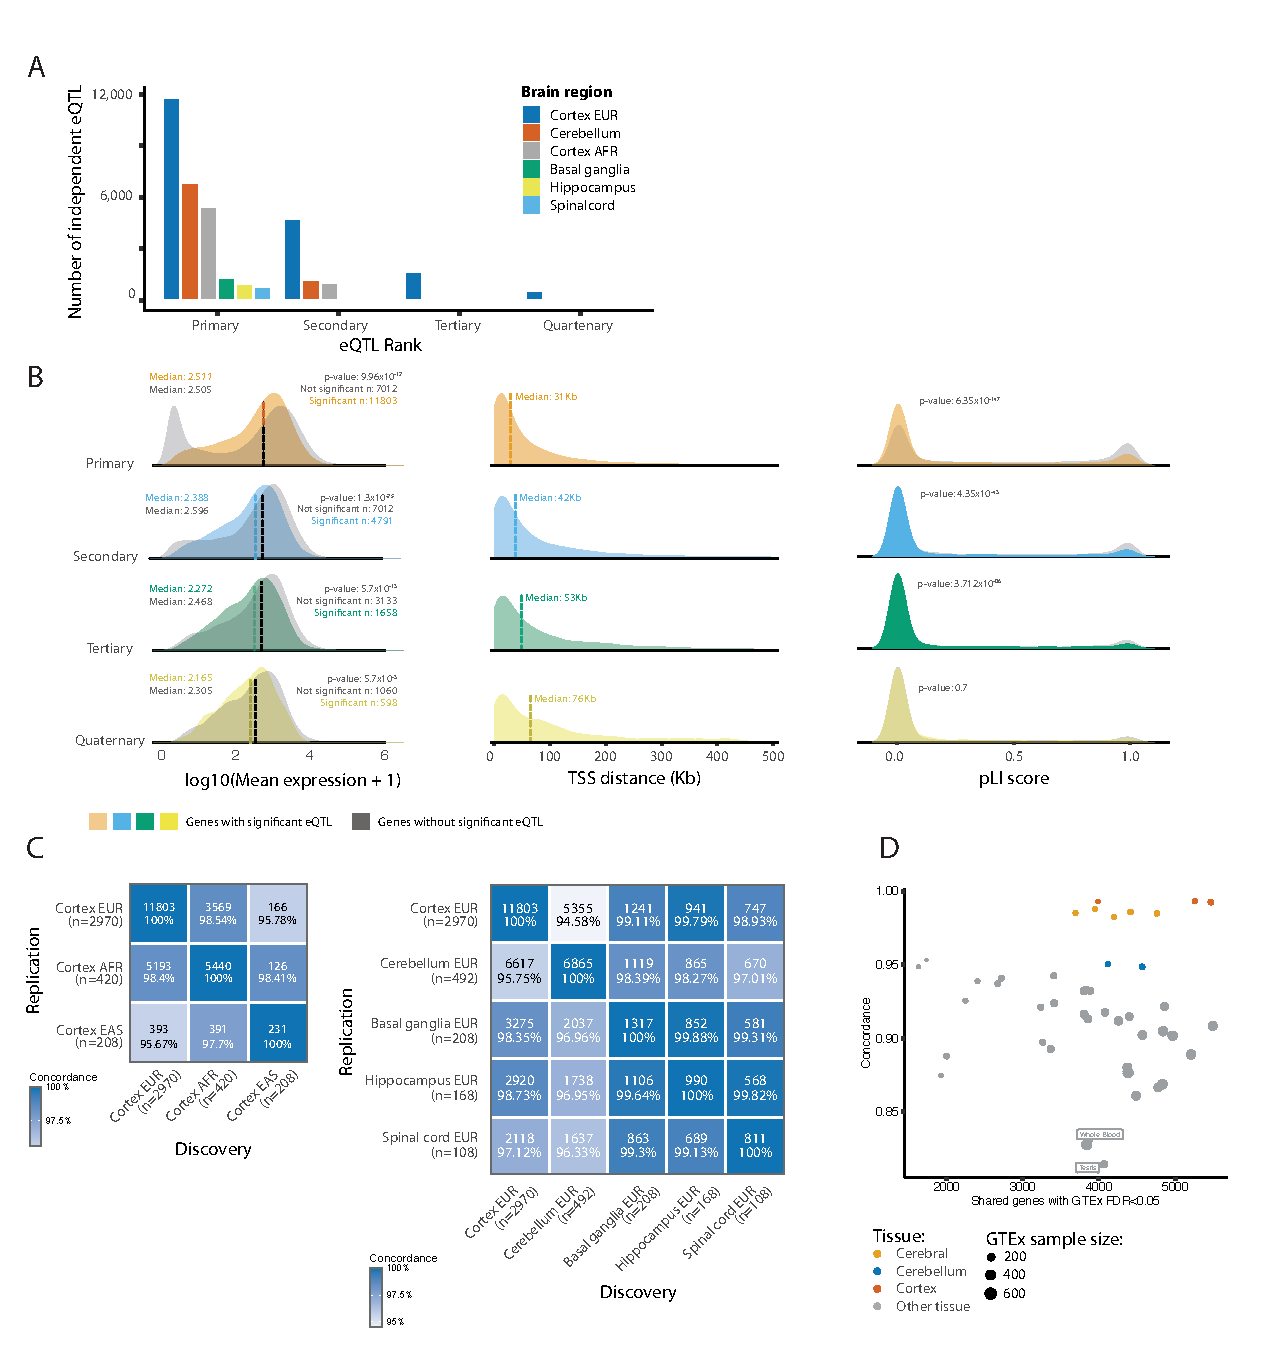
\includegraphics[width=\textwidth]{chapters/chapter5-brain-eqtls/img/2020-12-02-fig3-ciseqtls-v12.pdf}
	\caption{\textbf{Figure 3. Conditional \emph{cis}-eQTLs.} (A) The number of conditional \emph{cis}-eQTLs per eQTL dataset. (B) Replication of primary \emph{cis}-eQTLs between; (left) the cortex eQTLs of different ethnicities (left) and; (right) the different brain regions for the European datasets. The n under the dataset name is the number of samples in that dataset. The boxes show the number the number of eQTLs that are significant in both the discovery and the replication set, and the percentage of those that shows the same direction of effect. (C) The replication between primary \emph{cis}-eQTLs of Cortex-EUR (discovery) with all the GTEx tissues (replication). Each dot is a different GTEx tissue, the x-axis is the number of eQTLs that is signifcant in both discovery and replication, and the y-axis is the percentage that shows the same direction of effect. (D) Comparison of characteristics between primary and non-primary eQTLs. (left) The difference in mean expression; (middle) the difference in distance between the most significant SNP-gene combination; (right) the difference in pLI score.}
\end{figure}

\subsection{8\% of Cortex \emph{cis}-eQTLs are mediated by cell type proportion differences  }
Cell type dependent eQTLs can be identified in bulk RNA-seq data by performing cell type deconvolution and determining cell type interaction eQTLs (ieQTLs)\cite{donovanCellularDeconvolutionGTEx2020,glastonburyCellTypeHeterogeneityAdipose2019,raulaguirregamboaDeconvolutionBulkBlood2020}. We predicted five major cell types using single cell RNA-seq derived signature profiles\cite{zhengyuCellMapCharacterizingType}. Of these, neurons were the most abundant cell type (median cell proportion: 32.8\%), followed by endothelial cells (24.9\%), macrophages (17.8\%), oligodendrocytes (12.4\%), astrocytes (12.1\%; \textbf{Supplementary Figure 7}). We predicted similar proportions for cerebellum (\textbf{Supplementary Figure 7}) as well as other brain regions (\textbf{Supplementary Figures 22 and 23}). As expected, we observed that predicted cell proportions are different for spinal cord, showing a relatively low proportion of neuronal cells and high proportions of macrophage and oligodendrocytes compared to other brain tissues. Predicted cell type proportions in cortex and cerebellum were negatively correlated between neurons and other cell types, and between endothelial cells and macrophages (\textbf{Figure 4A}). Additionally, they had a comparable scale and were positively correlated with immunochemistry (IHC) counts for each cell type in the ROSMAP cohort (Spearman r$>$0.1; \textbf{Figure 4B})\cite{patrickDeconvolvingContributionsCelltype2020}, and positively correlated (Spearman r$>$0.71) as a whole. We note however that validation of these predictions is difficult, because of the limited number of samples with IHC counts, but also because IHC, bulk RNA-seq and snRNA-seq all reflect different aspects of gene or protein expression, and finally because of the lack of a consensus of the expected proportion for each cell type\cite{herculano-houzelHumanBrainNumbers2009,vonbartheldSearchTrueNumbers2016}. 

We next used DeconQTL\cite{raulaguirregamboaDeconvolutionBulkBlood2020} to identify interaction-eQTLs (ieQTLs) by testing 18,850 cis-eQTLs in Cortex-EUR and 8,347 \emph{cis}-eQTLs in cerebellum (including primary, secondary, tertiary and quaternary eQTLs). We identified 1,515 significant ieQTLs (8\%) in at least one cell type (Benjamini-Hochberg; BH FDR < 0.05) for Cortex-EUR (\textbf{Supplementary Table 2}). Of these, 632 (42\%) were an ieQTL in neurons, likely because this is the most prevalent cell type. The majority (90.2\%) of the ieQTLs were uniquely mapped to one cell type (\textbf{Figure 4C}). We observed a lower proportion of ieQTLs in cerebellum (126; 1.5\%, \textbf{Supplementary Figure 8, Supplementary Table 2}), most likely due to the smaller sample size. 55 (44\%) of these ieQTLs were mediated by astrocytes.  

We compared the allelic direction of the identified ieQTLs for each cell type with matching cell types from a single nucleus RNA-seq (snRNA-seq) dataset (ROSMAP cohort, n=39; \textbf{Supplementary Table 10})\cite{mathysSinglecellTranscriptomicAnalysis2019}. When filtering on cell-type mediated eQTLs by Decon-QTL (FDR < 0.05) we observed a high average concordance in allelic direction for both the eQTL main effect (68\%), as well as the direction of the interaction (68\%; \textbf{Supplementary Figure 20B}). In total we were able to significantly (BH FDR<0.05) replicate 106 primary cortex cis-eQTLs (63 in excitatory neurons and 43 in oligodendrocytes). Of these, 13 excitatory neuron and 21 oligodendrocyte ieQTLs were cell type mediated by the corresponding cell type in bulk (Decon-QTL; BH FDR < 0.05; \textbf{Supplementary Figure 20D}). We observed a 100\% allelic concordance for both cell types in this subset. The ieQTLs replicating in oligodendrocytes included \emph{STMN4}, \emph{NKAIN1}, and \emph{FAM221A} (\textbf{Supplementary Figure 25A, B, and C}), which have previously been identified as oligodendrocyte specific\cite{ngUsingTranscriptomicHidden2019}. Additionally, this set of ieQTLs included \emph{AMPD3} (rs11042811) and \emph{CD82} (rs2303865), which play a role in white matter microstructure\cite{zhaoLargescaleGWASReveals2019}, suggesting an important role for oligodendrocytes in this pathway. The ieQTLs replicating in excitatory neurons included \emph{SLC25A27} (alias \emph{UCP4}; \textbf{Supplementary Figure 25D}), a gene principally expressed in neuron cells\cite{smorodchenkoComparativeAnalysisUncoupling2009} in the central nervous system\cite{ramsdenHumanNeuronalUncoupling2012} and known to modulate, amongst others, neuronal energy metabolism\cite{liuMitochondrialUCP4Mediates2006}. The eQTL SNP for this gene, rs2270450, was in high LD ($R^2$=0.71) with a variant previously associated with schizophrenia\cite{yasunoSynergisticAssociationMitochondrial2007} and previous work has suggested a possible role of this gene in Parkinson’s Disease\cite{ramsdenHumanNeuronalUncoupling2012,hoMitochondrialNeuronalUncoupling2012}, both of these diseases have a major neuronal involvement. These results suggest that the sample size of \emph{MetaBrain} is sufficient to accurately decompose eQTLs to their relevant cell type. 

\subsection{Shared genetic effects between MetaBrain eQTLs and brain-related traits}
	
As one application of the \emph{MetaBrain} resource, we linked \emph{cis}-eQTLs to variants associated with neurological traits and diseases. For this, we first evaluated linkage disequilibrium (LD) between the Cortex-EUR \emph{cis}-eQTL SNPs with the strongest association signals and index variants identified in 3,217 GWASs of brain-related traits (\textbf{Supplementary Note, Supplementary Table 5}). We observed that 10\% of \emph{cis}-eQTL SNPs were in LD (r2$>$0.8, distance between SNPs $<$ 1Mb, LD calculations were performed in the EUR subset of CMC) with brain-related trait SNPs, involving 242 eQTL genes. This percentage marginally increased to 12\% when secondary, tertiary and quaternary eQTL SNPs were included, indicating that the majority of LD overlap is driven by primary eQTL effects. 

To more formally test for overlap between GWAS and eQTL signals, we next implemented a Mendelian Randomization (MR) analysis to test for a causal effect between gene expression and 31 neurological traits using cis-eQTLs as instruments (\textbf{Supplementary Table 7}).  For our MR analysis, we computed a Wald ratio for each eQTL instrument, from which 1,192 Wald ratios out of 268,030 tested in total passed our suggestive p-value threshold ($p<5 \times 10^{-5}$; \textbf{Supplementary Table 8}). However, inferring causality from a Wald ratio can be misleading as it is possible for the eQTL instrument to coincidentally share association with the GWAS trait due to surrounding LD patterns in the genomic region.  To confirm this is not the case, we further narrowed down our list of genes with evidence of Wald ratio effects by determining genetic colocalization between GWAS and \emph{cis}-eQTL signals using COLOC\cite{BayesianTestColocalisation}. This identified 159 significant Wald ratios that passed a strict Bonferroni correction ($p<1.87 \times 10^{-7}$) where the GWAS SNP and eQTL colocalized (PP4$>$0.7; \textbf{Table 2}; \textbf{Figure 5A}). Three examples where MR and colocalization pointed to likely causal GWAS genes are reported below, for others see \textbf{Supplementary Note}. 

\begin{figure}[H]
	\includegraphics[width=\textwidth]{chapters/chapter5-brain-eqtls/img/2020-11-25-fig4-interactionqtls-v8.pdf}
	\caption{\textbf{Cell type interacting eQTLs.} (A) Spearman correlation between the 5 predicted cell count proportions. Lower triangle is within Cortex samples, upper triangle is within Cerebellum samples. (B) Predicted cell count proportions (x-axis) versus measured cell count proportions (y-axis) for Cortex. Values in the plot are Pearson correlation coefficients. (C) Number of cell type interacting eQTLs for Cortex deconvoluted cell types. (D) Bulk eQTL (left) and cell type interacting eQTL (right) for ADAMTS18 interacting with predicted oligodendrocyte proportion.}
	\end{figure}

\subsection{MR and colocalization analysis involves \emph{TSPAN14} with Alzheimer’s disease }

\emph{TSPAN14} has recently been identified as an AD risk locus\cite{schwartzentruberGenomewideMetaanalysisFinemapping2020}. Our MR and colocalization analysis using rs10749609 as an eQTL instrument variable found higher expression of \emph{TSPAN14} as putatively causal for AD (MR Wald ratio=0.17, $p=6.7 \times 10^{-9}$; Coloc PP4 $>$ 0.95). ieQTL analysis did however not detect a significant interaction for the included cell type proportions. \emph{TSPAN14} interacts with \emph{ADAM10}​, which mediates proteolytic cleavage of more than 40 substrates including APP and TREM2\cite{matthewsRegulationLeukocytesTspanC82018}. Missense mutations in \emph{ADAM10} that attenuate its \alpha-secretase activity shift APP processing toward \beta-secretase-mediated cleavage, increase A\beta plaque load and reactive gliosis\cite{suhADAM10MissenseMutations2013}. Overexpression of \emph{TSPAN14} has been shown to increase cell surface expression of ADAM10\cite{jouannetTspanC8TetraspaninsDifferentially2016}, suggesting AD risk at this locus may be conferred through imbalanced \alpha- to \beta-secretase cleavage, although further experiments are needed to explain an apparent inverse directionality in our analyses. 

\subsection{MR and colocalization analysis links multiple sclerosis GWAS loci to cell type specific eQTLs for \emph{CYP24A1} and \emph{CLECL1}}
MR analysis for multiple sclerosis (MS) identified 157 instruments that passed the suggestive threshold of $p<5 \times 10^{-5}$, representing 135 unique genes (\textbf{Supplementary Table 8}). For 20 of these genes, our approach identified colocalization (\textbf{Table 2; Figure 5C}), including 11 genes for which MR suggested that increased gene expression and 9 genes where decreased gene expression leads to MS risk. Systematic comparison of the MR Wald ratio estimates for MS of 5,986 shared eQTL genes) between Cortex-EUR and eQTLGen (where the same gene was instrumented but could be with different SNPs)\cite{vosaUnravelingPolygenicArchitecture2018} showed opposite directions of effect for 2,373 (39.6\%) genes (\textbf{Supplementary Figure 24}).  Agreement improved when the same SNP instrument was compared on between studies but still remained high with 1,891 (26\%) out of 7,274 \emph{MetaBrain} Wald ratios showing opposite directionality to eQTLGen. Of the 135 genes with MR findings in Cortex-EUR for MS, we identified 29 genes without a significant eQTLgen instrument including 3 genes, \emph{SLC12A5}, \emph{CCDC155} and \emph{MYNN}, for which we found both MR significance and colocalization in \emph{MetaBrain}. (see \textbf{Supplementary Note; Supplementary Table 14}). The discrepancy in MR findings observed between Cortex-EUR and eQTLgen suggest tissue-dependent genetic effects for MS. 

Two MS genes, \emph{CYP24A1} and \emph{CLECL1}, showed cell-type specific eQTLs (\textbf{Figure 5D}). Our analysis used rs2259735 as the Cortex-EUR eQTL instrument variable and suggested higher expression of CYP24A1 is associated with increased MS risk for the C-allele (MR Wald ratio= 0.13, $p=1.7 \times 10^{-9}$. We also observed colocalization of the eQTL and the MS GWAS signal at this region (Coloc PP4=0.99), suggesting the same underlying genetic signal. Furthermore, ieQTL analysis showed increasing expression of \emph{CYP24A1} with increasing neuronal proportions for the MS risk allele rs2248137-C (interaction FDR=$p=1 \times 10^{-308}$; \textbf{Figure 4E}). Rs2248137 has previously been associated with MS\cite{consortiumMultipleSclerosisGenomic2019} and is in strong LD with SNP rs2259735 (r2=0.9). \emph{CYP24A1} is a mitochondrial cytochrome P450 hydroxylase that catalyzes the inactivation of 1,25-dihydroxyvitamin D3 (calcitriol), the active form of vitamin D\cite{jones25HydroxyvitaminD24hydroxylaseCYP24A12012}. Loss of function mutations in \emph{CYP24A1} increase serum calcitriol and cause hereditary vitamin D-mediated PTH-independent hypercalcemia\cite{schlingmannMutationsCYP24A1Idiopathic2011,cappellaniHereditaryHypercalcemiaCaused2019}. In the brain, vitamin D plays vital functions in regulating calcium-mediated neuronal excitotoxicity, reducing oxidative stress, and regulating synaptic activity\cite{mpandzouVitaminDeficiencyIts2016}. Epidemiological studies have proposed vitamin D deficiency as a risk factor for MS\cite{agnelloCYP27A1CYP24A1RXRalpha2018,pierrot-deseillignyHypovitaminosisOneEnvironmental2010}, which has recently been validated through MR\cite{rheadMendelianRandomizationShows2016,jacobsBMILowVitamin2020,jiangCausalRoleCirculating2021}.  Our findings are consistent with a previous report of a shared MS GWAS signal and \emph{CYP24A1} eQTL signal in the region with frontal cortex but not white matter, using brain eQTL data sets derived from expression microarrays to confirm the findings in the same direction of effect\cite{ramasamyGeneticEvidencePathogenic2014}.  

As another MS signal that passed MR and colocalization, decreased expression of \emph{CLECL1} is associated with increased MS risk (MR Wald ratio=-0.16, $p=1.58 \times 10^{-9}$, Coloc PP4$>$0.92). The ieQTL analysis indicated that the rs7306304-A allele increased expression of \emph{CLECL1} with increasing macrophage proportion (interaction FDR=$1 \times 10^{-308}$, \textbf{Figure 4F}). Rs7306304 is in strong LD with the MS lead SNP, rs7977720 (r2=0.84)\cite{consortiumMultipleSclerosisGenomic2019}. \emph{CLECL1} encodes a C-type lectin-like transmembrane protein highly expressed in dendritic and B cells that has been proposed to modulate immune response\cite{vanluijnMultipleSclerosisassociatedCLEC16A2015}. While \emph{CLECL1} expression was low in cortical bulk RNA-seq data, it had a 20-fold higher expression in purified microglia\cite{consortiumMultipleSclerosisGenomic2019}, suggesting that decreased \emph{CLECL1} expression increases MS susceptibility through microglia-mediated dysregulation of immune processes in the brain. 

\begin{figure}[H]
	\includegraphics[width=\textwidth]{chapters/chapter5-brain-eqtls/img/2020-12-02-fig6-ms-v2.pdf}
	\caption{\textbf{Figure 6.}(C) Cell type interacting eQTL for CYP24A1 (top) and CLECL1 (bottom) interacting with predicted neuron, and macrophage proportion respectively. }
\end{figure}

\subsection{87\% of trans-eQTLs are located in the 7p21.3 \emph{TMEM106B} locus }
Disease associated variants can also act on distal genes through trans-eQTLs. To maximize sample size, we performed \emph{trans}-eQTL analysis meta-analyzing Cortex-EUR and Cortex-AFR together (n=3,111; SNP distance to TSS$>$5Mb), while leaving out ENA to prevent bias by genotypes called from RNA-seq samples. For this analysis, we did not correct for 10 PCs, since trans-eQTLs can be driven by cell proportion differences\cite{vosaUnravelingPolygenicArchitecture2018}, and these PCs were correlated with estimated cell type proportions (\textbf{Supplementary Figure 26}). We reduced the number of tests performed by limiting this analysis to 145,413 variants that are likely to affect gene expression in \emph{trans}: variants that have been associated with diseases and traits through GWAS and variants that were primary and non-primary \emph{cis}-eQTLs from any of the discovery datasets.  

We identified 3,940 \emph{trans}-eQTLs (FDR$<$0.05), of which 2,589 (66\%) were significant after correcting for genes that likely cross map within 5Mb of the \emph{trans}-eQTL SNP (\textbf{Figure 6A}). These 2,589 eQTLs reflected 373 unique SNPs, and 1,263 unique genes. Of these 2,589 \emph{trans}-eQTLs, we were able to replicate 21 in snRNA-seq of excitatory neurons with 100\% allelic concordance (\textbf{Supplementary Figure 21; Supplementary Table 11}). While this number of replicating \emph{trans}-eQTLs is low due to the small sample size of the snRNA-seq dataset, it is unlikely that these 21 \emph{trans}-eQTLs are driven by cell type proportion differences, since they were detected in a single cell type. 

222 (60\%) of the \emph{trans}-eQTL SNPs were also a significant cis-eQTL SNP in the Cortex-EUR analysis. 83 (22\%) were also the index SNP for a \emph{cis}-eQTL, of which 42 (51\%) in Cortex-EUR, and 22 (27\%) in tissues other than cortex. This suggests that trans-eQTLs can also be observed for cis-eQTLs index SNPs identified in other tissues.  

We observed 14 genes on which multiple independent genomic loci had a convergent trans-eQTL. The variants involved in these convergent trans-eQTL effects were previously associated with blood and immune related phenotypes (\emph{ANKRD2}, \emph{HBG2}, \emph{PIWIL2}, \emph{PROM1}, \emph{SVEP1}), neurological phenotypes (\emph{DAZAP2}), both immune and neurological phenotypes (\emph{HMCES}, \emph{KCNA5}, \emph{MBTPS1}, \emph{PRPF19}, \emph{PTH2R}, \emph{RFPL2}), or other phenotypes (\emph{PEX12}, \emph{PIWIL2}, \emph{ZNF727}). For example, two independent variants (rs1427407 and rs4895441) affected \emph{HBG2} (11p15.4) in \emph{trans} (\textbf{Figure 6B}). rs1427407 (2p16.1) is located in an intron of the \emph{BCL11A} gene, although we did not observe a \emph{cis}-eQTL in this locus. rs4895441 (6q23.3) had a cis-eQTL on the \emph{ALDH8A} and \emph{HBS1L} genes in Cortex-EUR. The three loci in which these genes reside have previously been associated with fetal hemoglobin levels\cite{sankaranHumanFetalHemoglobin2008,jiangCMYBInvolvedRegulation2006,metaisGenomeEditingHBG12019} and various blood cell counts, while the 6p23.3 locus has also been associated with adult height\cite{wojcikGeneticAnalysesDiverse2019}.  

All convergent \emph{trans}-eQTLs were affected by two independent loci, except \emph{KCNA5}s (12p13.32), which was affected by variants from three independent loci (\textbf{Figure 6B}): rs930263 (2p23.3), rs2702575 and rs2604551 (4p15.32), and rs10950398 and rs11974335 (7p21.3). \emph{KCNA5} encodes the potassium voltage-gated channel protein Kv1.5. Potassium voltage-gated channels regulate neuron excitability among other functions, and blockers for these channels have been suggested as a therapeutic for multiple sclerosis patients\cite{jDalfampridineBriefReview2011}. Furthermore, \emph{KCNA5} has previously been associated with cardiovascular disease\cite{al-owaisMultipleMechanismsMediating2017}, and has been suggested to modulate macrophage and microglia function\cite{rusVoltagegatedPotassiumChannel2005}. Three \emph{cis}-eQTLs were associated with rs930263, including \emph{ADGRF3}, \emph{DRC1}, and a secondary eQTL on \emph{HADHB}. rs930263 was previously associated with sleep dependent LDL levels\cite{noordamMultiancestrySleepbySNPInteraction2019} and several blood metabolite levels\cite{galloisComprehensiveStudyMetabolite2019,sunGenomicAtlasHuman2018,suhreConnectingGeneticRisk2017,tinTargetGenesVariants2019}. The locus on 4p15.32 was previously associated with insomnia and adult height\cite{kichaevLeveragingPolygenicFunctional2019}, and the 7p21.3 locus with depression and blood protein levels. These results thus suggest that several sleep related variants affect potassium voltage-gated regulation of neuron excitability.  

2,252 (87\%) of the observed \emph{trans}-eQTL genes were affected by a set of 45 variants that were all located at 7p21.3 (\textbf{Figure 6A}). This locus is associated with many traits, including brain-related phenotypes, such as frontotemporal dementia and major depressive disorder and non-neurological phenotypes such as blood protein levels and height. The majority (81\%) of these \emph{trans}-eQTLs were associated with two SNPs, rs11974335 and rs10950398 ($R^2$=0.98), which are both located in an intron of \emph{TMEM106B} and were associated with 1,025 and 790 genes, respectively (\textbf{Figure 6C}). While we did not observe a \emph{TMEM106B} \emph{cis}-eQTL for any variant in the locus, we did observe \emph{cis}-eQTLs for 22 other genes. Of note, this included rs1990622 ($R^2$=0.96 with rs11974335), an index variant for frontotemporal lobar degeneration\cite{liGeneticVariantsAssociated2018} (FTLD) located downstream of \emph{TMEM106B}, which had a \emph{cis}-eQTL on \emph{THSD7A} (SNP–TSS distance $>$ 411kb; \textbf{Figure 6C}). The FTLD risk allele rs1990622-A decreased expression of this gene, which is suggested to be involved in neuro-angiogenesis\cite{kuoSolubleTHSD7ANGlycoprotein2011} (\textbf{Figure 6D}). rs1990622 was associated with 35 \emph{trans}-eQTL genes, of which 31 were negatively regulated by the FTLD risk allele (\textbf{Supplementary Figure 29}). Downregulated genes included genes involved in calcium transport such as \emph{CALB2}, and \emph{CBLN1}, and potassium transport, such as \emph{KCND3}, \emph{KCHN5} and \emph{KCDT2} (\textbf{Figure 6C, Figure 6D}). Collectively, upregulated trans-eQTL genes for rs11974335, rs10950398 and rs1990622 were enriched for neuron related processes, such as synaptic signaling (p=$p=1.3 \times 10^{-28}$) and nervous system development ($p=2.9 \times 10^{-21}$), while downregulated genes were enriched for gliogenesis ($p=1.6 \times 10^{-8}$) and oligodendrocyte differentiation ($p=3.1 \times 10^{-6}$). 

While rs11974335 and rs10950398, rs1990622 are in high LD (R2$>$0.9), we observed only a limited number of \emph{trans-eQTL genes for rs1990622. rs11974335 and rs10950398 were tested in only 6 datasets with WGS derived genotypes, while rs1990622 was tested in 20 datasets, suggesting that heterogeneity between datasets decreased the number of significant \emph{trans}-eQTLs for rs1990622 (\textbf{Figure 6D}). Indeed, \emph{trans}-eQTLs for rs1990622 were highly heterogeneous across the included datasets, being most pronounced in the AMP-AD and UCLA\_ASD datasets, and less so in other datasets of comparable sample size, such as CMC. As another potential source for heterogeneity, we considered that many of the observed \emph{trans}-eQTLs might be driven by differences in cell type proportions. We therefore associated the five predicted cell type proportions with genotypes and identified 142 associations from 122 variants (FDR$<$0.05), of which 116 were located in the 7p21.3 locus. This included rs1990622, which showed a decrease in neuron proportions for the FTLD risk allele, matching previous reports (\textbf{Figure 6D}). Like the observed \emph{trans}-eQTLs, these neuron proportion associations were most pronounced in the AMP-AD datasets. However, when comparing average neuron proportions in AMP-AD with those in other datasets, we did not observe many significant differences. Nevertheless, we observed a strong association between the correlation of \emph{trans}-eQTL gene expression levels and neuron proportions and the \emph{trans}-eQTL Z-scores (R2$>$0.85; Figure 6E). Comparing Alzheimer cases versus controls in the AMP-AD dataset, we observed that neuron proportions were significantly lower (\textbf{Figure 6F; Supplementary Figure 30}) and that \emph{trans}-eQTL Z-scores were higher (\textbf{Figure 6G}). This indicates that the observed \emph{trans}-eQTLs and neuron associations may be in part driven Alzheimer dependent loss of neurons, driven by the 7p21.3 locus. While our analysis cannot disentangle the neuron loss from the Alzheimer association at rs1990622, it does suggest that this locus affects many downstream genes in Alzheimer patients. 

\begin{figure}[H]
	\includegraphics[width=\textwidth]{chapters/chapter5-brain-eqtls/img/2020-10-19-fig5-ftd-v6.pdf}
	\caption{\textbf{Clustering and enrichment of \emph{trans}-eQTL genes of the ftd locus.} (A) Heatmap of the spearman correlation between 790 \emph{trans}-eQTL genes from the ftd locus. Separation of rows indicates the 3 major clusters. (B) Functional enrichment of cluster 1, cluster 2, and cluster 3 from (A). Dots show the p-value from g:profiler. Some of the HPO terms have been highlighted.on.}
\end{figure}

\subsection{Brain co-regulation networks improve GWAS interpretation}
We subsequently generated brain-region specific co-regulation networks based on the RNA-seq data from the 8,727 samples. We previously have done this for a heterogenous set of expression samples\cite{persBiologicalInterpretationGenomewide2015,deelenImprovingDiagnosticYield2019}, which showed that such a co-regulation network can be informative for interpreting GWAS studies\cite{persBiologicalInterpretationGenomewide2015} and helpful in the identification of new genes that cause rare diseases\cite{deelenImprovingDiagnosticYield2019}. 

Here we developed a new approach (‘Downstreamer’ in preparation, see \textbf{Supplementary Note}) that improves upon our previous method ‘DEPICT’: Downstreamer can systematically determine which genes are preferentially co-regulated with genes that reside within GWAS loci. It does not use a significance threshold for a GWAS, but uses all SNP information, accounts for LD and uses rigorous permutation testing to determine significance levels and control type 1 errors. 

We applied Downstreamer to schizophrenia, Parkinson’s disease, multiple sclerosis, Alzheimer’s disease and amyotrophic lateral sclerosis, and used a co-regulation network that was based on all 8,727 brain samples, a co-regulation network limited to cortex samples, and a co-regulation limited to cerebellum samples. 

We observed that there were multiple sets of genes that showed strong co-regulation with genes inside the GWAS loci for these diseases. For MS and Alzheimer’s disease, these were mostly immune genes, whereas for Parkinson’s disease, ALS and schizophrenia these were genes that are specifically expressed in brain. For ALS we identified a limited set of co-regulated genes, but observed that these genes are predicted to cause gait disturbance when mutated, when using our recently developed clinical symptom prediction algorithm\cite{deelenImprovingDiagnosticYield2019}. 

These results indicate that these genes do share clear biological relationships for diseases such as ALS, where various loci have been found for both familial and sporadic forms but for which it has not been clear what the mechanism is for many of the positional candidate genes: some other genes show strong co-regulation with genes inside these ALS loci, indicating that many positional candidate genes have a shared biological function. Finally, these identified co-regulated genes could well represent downstream targets that in the future might prove useful as potential pharmaceutical targets. 

\section{Discussion}

We have described an integrated analysis of the effects of genetic variation on gene expression levels in brain in over 3,000 unique individuals. This sample size yielded sufficient statistical power to identify weak \emph{cis}-eQTL and to our knowledge for the first-time brain \emph{trans}-eQTLs that emanate from SNPs that have been previously linked to neurodegenerative or psychiatric phenotypes. 

We compared the \emph{cis}-eQTLs in MetaBrain to \emph{cis}-eQTLs in eQTLgen, a set of 31,684 blood samples. We observe a large proportion of shared \emph{cis}-eQTLs between brain and blood, most of which have the same allelic direction of effect. Our analysis also permitted us to identify \emph{cis}-eQTL effects that are independent of the primary \emph{cis}-eQTLs. These secondary, tertiary and quaternary eQTLs are rarely shared with blood eQTLs. Some of these independent effects reflect SNPs that are also the index variants for several neurological and psychiatric disorders, making them particularly interesting for subsequent follow-up. Recent observations have revealed that strong \emph{cis}-eQTL effects are often observed for SNPs that are depleted for GWAS associations44. Since primary \emph{cis}-eQTLs often have such large-effect sizes, the secondary, tertiary and quaternary \emph{cis}-eQTL SNPs are therefore potentially more interesting to follow-up, as compared to some primary \emph{cis}-eQTL SNPs. 

LD overlap analysis, Mendelian randomization and colocalization are sensitive to many factors, including eQTL and GWAS study sample size, effect size, variant density, LD structure, and imputation quality. Differences between study designs may consequently influence the results of such analyses. For example, our colocalization and LD overlap analysis did not identify overlap between Alzheimer’s disease and the \emph{MAPT} gene, because the effect sizes of the \emph{cis}-eQTLs for this gene were limited in our study, with the lead SNP having an FDR corrected p-value of 0.02. Previous studies have been contentious, with some finding strong effects\cite{wangComprehensiveFunctionalGenomic2018,ngXQTLMapIntegrates2017} while others find weak or no effects within this locus\cite{aguetGeneticEffectsGene2017,siebertsLargeEQTLMetaanalysis2020}. The \emph{MAPT} locus is characterized by the presence of different long-range haplotypes, represented as three alternate sequences in the human genome reference (GRCh38) for this region, each containing a copy of the \emph{MAPT} gene with a different Ensembl gene identifier. When investigating the alignment of RNA-seq reads in this region, we observed that reads aligned to these alternate copies of MAPT introduced an eQTL on the reference copy of the gene, suggesting that the \emph{MAPT} eQTL was possibly caused by alignment bias rather than true biological effect (\textbf{Supplementary Note}). We note that this might be an issue for other genes as well. Future studies using graph-based alignment tools or long read sequencing methods would be required to ultimately determine the true effects on such genes. 

We studied different regions in the brain, permitting us to identify brain-region specific eQTLs as well. It is possible that some of these differences can be attributed to differences in cell-type proportions across different brain regions. We therefore first inferred cell-type percentages for the major cell-types that exist within brain. We then applied an eQTL interaction model (i.e. using the cell-type percentage x genotype as interaction term), permitting us to identify over 1,700 \emph{cis}-eQTL genes that show cell-type specificity, and could help better inform in what specific cell-type disease-associated variants show regulatory effects. Most of these cell-type dependent effects were observed for oligodendrocytes and neurons, the two most common cell types in the brain, and for which statistical power is therefore strongest to observe such effects. Still, we could identify cell-type dependent eQTLs for approximately 800 to macrophages, endothelial cells or astrocytes. Since these analyses were based on a deconvolution approach, these results remain to be validated in purified cell-types, e.g. from population-based single-cell RNA-seq datasets that are now becoming more commonplace\cite{wijstSinglecellRNASequencing2018,PopulationscaleSinglecellRNAseq}. Such single-cell eQTL studies can gain substantial statistical power by limiting analyses to the large set of primary, secondary, tertiary and quaternary \emph{cis}-eQTLs from our strongly powered study in bulk brain samples. 

This is the best powered Mendelian randomization and colocalization analysis using brain cis-eQTLs as instruments for bipolar disease, epilepsy, frontotemporal dementia, multiple sclerosis, fluid intelligence and years of schooling GWAS outcomes conducted to date in our knowledge. Interestingly, we also find three significant MR findings that passed colocalization for schizophrenia that were not reported in the latest publication from the PGC consortium for \emph{CILP2}, \emph{MAU2} and \emph{TM6SF2}\cite{consortiumMappingGenomicLoci2020}, further noting the value of having a well-harmonized, large eQTL data set in the tissue type of interest (\textbf{Supplementary Note}). We confirm by MR using Cortex-EUR \emph{cis}-eQTL instruments and colocalization that higher expression of \emph{TSPAN14} leads to Alzheimer’s disease. Our results also suggest that increased \emph{CYP24A1} expression leads to multiple sclerosis and implicate that neurons could be the most susceptible cell type to \emph{CYP24A1} expression changes and active vitamin D levels. This unelucidated role of \emph{CYP24A1} in the brain could play an important role in MS etiology. Additionally, our MR and colocalization findings suggest that insufficient expression of \emph{CLECL1} in microglia may increase MS disease risk.

The identified 2,589 \emph{trans}-eQTLs allow us to gain insight into the more downstream molecular consequences of several disease-associated genetic variant as well. We observed that variants that are brain \emph{cis}-eSNP more often give \emph{trans}-eQTL effects than expected by chance, indicating that \emph{cis}-eQTL effects often manifest themselves downstream as well. We identified for several SNPs, associated to neurological and psychiatric diseases such \emph{trans}-eQTLs that are helpful for better understanding the effect of such risk alleles. 

With more results coming out of GWAS, revealing ever more associated loci, interpretation of the downstream consequences of these variants is the next challenge. In this post-GWAS era our resource is particularly useful for researchers in the field of neurology and psychiatry. Our approach can be applied to many other tissues and fields of research to prioritize therapeutic targets from GWAS analysis. To our knowledge, this is the largest non-blood eQTL analysis ever conducted, providing insight into the functional consequences of many disease associated variants. We expect that through future integration with single-cell eQTL studies that have higher resolution but lower power, our results will help to pinpoint transcriptional effects in specific brain cell-types for many disease-associated genetic variants. 

\section{Material \& Methods}
\subsection{Dataset collection and description }
We collected human brain bulk RNA-seq datasets from different resources. Briefly, we collected previously published samples from the AMP-AD consortium (AMP-AD MAYO\cite{hodesAcceleratingMedicinesPartnership2016}, ROSMAP\cite{hodesAcceleratingMedicinesPartnership2016} and MSBB\cite{hodesAcceleratingMedicinesPartnership2016}) and the PsychENCODE consortium (Bipseq2, BrainGVEX2, CMC78, GVEX, LIBD, and UCLA\_ASD2) from Synapse.org using the Python package synapseclient\cite{teamSynapseclientClientSynapse}. For scripts including the synapse IDs downloaded see \url{https://github.com/npklein/brain\_eQTL/tree/master/synapse\_download\_scripts}. The NABEC and GTEx datasets were retrieved from NCBI dbGaP (phs001301.v1.p1, phs000424.vN.pN), and TargetALS was retrieved through personal communication. For an overview of the number of samples per dataset, see \textbf{Supplementary Table 1}. 

Additionally, we collected public brain bulk RNA-seq samples from the European Nucleotide Archive (ENA). To select only the brain samples, we first downloaded the SkyMap database\cite{tsuiExtractingAllelicRead2018}, which provides readily mapped read counts and sample annotations. We performed rigorous quality control on this dataset, and selected ENA, excluding for example brain cell lines, brain cancer samples, and samples with RNA spike ins (See \textbf{Supplementary Note} for more details on this method, \textbf{Supplementary Figure 9}), resulting in xyz samples, and xyz samples when combined with the previously published datasets. 

\subsection{RNA-seq data}
RNAseq data was processed using a pipeline built with molgenis-compute\cite{byelasMOLGENISBasedComputational2011}. FastQ files were aligned against the GENCODE\cite{frankishGENCODEReferenceAnnotation2019} v32 primary assembly with STAR\cite{dobinSTARUltrafastUniversal2013} (version 2.6.1c), while excluding patch sequences (see \textbf{Supplementary Note}) with parameter settings: outFilterMultimapNmax = 1, twopassMode Basic, and outFilterMismatchNmax = 8 for paired-end sequences, outFilterMismatchNmax = 4 for single-end sequences. Gene quantification was performed by STAR, similar to gene quantification using HTSeq\cite{andersHTSeqPythonFramework2015} with default settings. The gene counts were then TMM\cite{robinsonScalingNormalizationMethod2010} normalized per cohort using edgeR\cite{robinsonEdgeRBioconductorPackage2010} (version 3.20.9) with R\cite{rcoreteamLanguageEnvironmentStatistical2017} (version 3.5.1). 

To measure FastQ and alignment quality we used FastQC\cite{BabrahamBioinformaticsFastQC} version 0.11.3), STAR metrics, and Picard Tools\cite{broadinstitutePicardTools2019} (version 2.18.26) metrics (MultipleMetrics, and RNAseqMetrics). Samples were filtered out if aligned reads had $<$ 10
\% coding bases (\textbf{Supplemental Figure 10A}), $<$ 60\% reads aligned (\textbf{Supplemental Figure 10B}), or $<$ 60\% unique mapping. 117 of the RNA-seq samples did not pass this filter, mostly from GTEx\cite{consortiumGTExConsortiumAtlas2020}. The other quality measurements were visually inspected but contained no outliers. 

RNA-sequencing library preparation, and other technical factors can greatly influence the ability to quantify of gene expression. Therefore, for a given sample such factors often influence the total variation. For example, such issues can be caused by problems during RNA-seq library preparation that lead to an increased number of available \emph{trans}cripts to quantify, or conversely, a lack of variation in quantified \emph{trans}cripts (compared to other samples in the dataset). We therefore opted to identify RNA-seq outliers that were not explained by poor RNA-seq alignment metrics. For this purpose, we performed PCA on the RNA data prior to normalization: we reasoned that the first two components capture excess or depletion of variation caused by technical problems. We identified 20 RNA-seq outliers with PC1 score $>$4 standard deviation away from the mean (\textbf{Supplementary Figure 11A}). After removal of these 20 outlier samples the PCs were recalculated (\textbf{Supplementary Figure 11B}). We then again removed 45 samples where the PC1 score was 4 standard deviations away from the mean and recalculated the PCs confirming no additional samples had outlier PC1 scores (\textbf{Supplementary Figure 11C}) leaving 3,677 samples for further analysis. 



We next removed genes with no variation and then log2-transformated, quantile normalized, and Z-score \emph{trans}formed the RNA-seq counts per sample. PCA on the normalized expression data showed that datasets strongly cluster together (\textbf{Supplementary Figure 12A}), likely due to dataset specific technical differences (e.g. single-end versus paired-end sequencing). To correct for this the normalized expression data was correlated against 77 covariates from different QC tools, such as percent protein coding, GC content, and 5’ prime/3’ prime bias. The top 20 correlated technical covariates (\% coding bases, \% mRNA bases, \% intronic bases, median 3’ prime bias, \% usable bases, \% intergenic bases, \% UTR bases, \% reads aligned in pairs, average mapped read length, average input read length, number of uniquely mapped reads, \% reads with improper pairs, number of reads improper pairs, total sequences, total reads, \% chimeras, number of HQ aligned reads, number of reads aligned, HQ aligned Q20 bases, HQ aliged bases) were regressed out of the expression data using a linear model. After covariate correction, clustering of datasets in PC 1 and PC 2 was no longer present (\textbf{Supplementary Figure 12B}).  

Our collection of RNA-seq samples consisted of 36 different tissue labels, many of which were represented by only a few samples. Therefore, we next defined major brain regions present in our dataset, including samples from amygdala, basal ganglia, cerebellum, cortex, hippocampus and spinal cord. We noted that some samples (especially from ENA) were not annotated with a specific major brain region. To resolve this, we performed PCA over the sample correlation matrix and then performed k-nearest neighbors on the first two PCs (k=7) to classify samples to the major brain regions. Using this approach, we defined a set of 86 amygdala, 574 basal ganglia, 723 cerebellum, 6,601 cortex, 206 hippocampus, 252 hypothalamus and 285 spinal cord samples (\textbf{Supplementary Table 1}, \textbf{Figure 2A}). 



\subsection{Genotype data and definition of eQTL datasets}
The genotype data for the included datasets was generated using different platforms, including genotypes called from whole genome sequencing (WGS; AMP-AD, TargetALS, GTEx\cite{consortiumGTExConsortiumAtlas2020}), genotyping arrays (NABEC, Braineac\cite{ramasamyGeneticVariabilityRegulation2014}), and haplotype reference consortium (HRC)\cite{mccarthyReferencePanel642016} imputed genotypes (PsychENCODE datasets), or were called from RNA-seq directly (ENA dataset; see Supplementary Note). In total, 22 different genotyping datasets were available, reflecting 6,658 genotype samples (\textbf{Supplementary Table 1}).  

We performed quality control on each dataset separately, using slightly different approaches per platform. For the array-based datasets, we first matched genotypes using GenotypeHarmonizer\cite{deelenGenotypeHarmonizerAutomatic2014} using 1000 genomes phase 3 v5a (1kgp) as a reference, limited to variants having MAF $>$ 1\%, $<$ 95\% missingness and Hardy-Weinberg equilibrium p-value $<$ 0.0001. Genotypes were then imputed using HRC v1.1 as a reference on the Michigan imputation server 30. In all HRC imputed datasets, variants with imputation info score $<$ 0.3 were removed. For the WGS datasets, we removed indels and poorly genotyped SNPs having VQSR tranche $<$ 99.0, genotype quality $<$ 20, inbreeding coefficient $<$ -0.3 and $>$ 5\% missingness, setting genotype calls with allelic depth < 10 and allelic balance $<$ 0.2 or $>$ 0.8 as missing. WGS datasets were not imputed with HRC. Considering the small size of some of the datasets, we decided to focus further analysis on variants with MAF $>$ 1\% and Hardy-Weinberg p-value $>$ 0.0001. 

In each dataset, we removed genetically similar individuals by removing individuals with pihat $>$ 0.125, as calculated with Plink. Additionally, we merged genotypes with those from 1kgp, pruned genotypes with --indep-pairwise 50 5 0.2 in plink, and performed PCA on the sample correlation matrix. We performed k-nearest neighbors (k=7) on the first two PCs, using the known ancestry labels in 1kgp, to assign an ancestry to each genotyped sample. The majority of included samples was of EUR descent: 5,138 samples had an EUR assignment, 805 samples had an AFR assignment, and 573 samples were assigned to the other ethnicities (\textbf{Supplementary Table 1}, \textbf{Figure 2B}). 

For the purpose of eQTL analysis, we next assessed links between RNA-seq and genotype samples and noted that some individuals had multiple RNA-seq samples (e.g. from multiple brain regions) or multiple genotype samples (e.g. from different genotyping platforms). In total, we were able to determine 7,644 links between RNA-seq samples and genotype samples (Supplementary Table 1), reflecting 3,525 unique EUR individuals, 624 unique AFR individuals, and 510 unique individuals assigned to other ethnicities. We then grouped linked RNA-seq samples based on ethnicity and tissue group to prevent possible biases on eQTL results. For those individuals with multiple linked RNA-seq samples, we selected a sample at random within these groups. Within each tissue and ethnicity group, we then selected unique genotype samples across datasets in such a way to maximize sample size per genotype dataset. For the eQTL analysis per tissue, we only considered those datasets having more than 30 unique linked samples available, and for which at least two independent datasets were available. Using these criteria for sample and dataset selection, we were able to create 7 eQTL discovery datasets: Basal ganglia-EUR (n=208), Cerebellum-EUR (n=492), Cortex-EUR (n=2,970), Cortex-AFR (n=420), Hippocampus-EUR (n=168) and Spinal cord-EUR (n=108; \textbf{Supplementary Table 1}, \textbf{Figure 2C}). 

\subsection{Gene co-regulation network}
For the gene co-regulation network, gene expression was quantified using Kallisto\cite{brayNearoptimalProbabilisticRNAseq2016} (version 0.43.1) to be in line with the gene expression quantification for the gene co-regulation network as described by Deelen \emph{et al.}\cite{deelenImprovingDiagnosticYield2019}  CRAM files created during RNA-seq processing for the eQTL analysis were converted to FastQ files using SAMtools\cite{liSequenceAlignmentMap2009} (version 1.9). Quantification was done against the Ensembl\cite{cunninghamEnsembl20192019} v98 \emph{trans}criptome with the patch chromosomes removed. The index was built using default options, with k-mer size = 31. For both paired-end and single-end samples the –bias option was used. For the paired-end samples all other options used default values. For single-end samples –fragment-length=200, and –sd=20 were used, for all other options the default values were used. 

After \emph{trans}cript quantification, \emph{trans}cript counts were summed to gene counts using Gencode\cite{frankishGENCODEReferenceAnnotation2019} v32 primary assembly GTF for \emph{trans}cript to gene mapping.  Genes that showed zero variance over all samples were removed for further analysis. Raw counts were quantile normalized before running PCA analysis to identify and remove possible outliers, but no outliers were detected, likely because only samples that passed the quality control for the eQTL analysis were included. Subsequently, raw counts were normalized by DESeq’s\cite{loveModeratedEstimationFold2014} median of ratios method before technical covariates identified for the eQTL analysis were removed. From the DESeq\cite{loveModeratedEstimationFold2014} normalized and covariate removed expression data a gene-gene Pearson correlation matrix was calculated and eigenvector and eigenvalues were calculated on this matrix using eigenvalue decomposition. The eigenvectors were centered and scaled and a gene-gene Pearson correlation matrix was calculated on the eigenvector matrix. 

For 6 types of gene set databases (KEGG, REACTOME, HPO, GO Molecular Function, GO Biological Process, and GO Cellular Component) coregulation and gene set predictions were calculated with GeneNetwork. The gene set predictions use the number of eigenvectors to include as a parameter. To determine the optimal number of eigenvectors to use we repeated the gene set predictions for n eigenvectors between 25-1000 with steps of 25, and 1000-2000 with steps of 200, and for each gene set database selected the number of eigenvectors with the highest mean AUC (\textbf{Supplementary Figure 13}). Heatmaps of the Pearson correlation of the AUC values between different steps shows that there is not much difference in AUC’s once a certain number of eigenvectors has been reached (generally around 100-225 eigenvectors, \textbf{Supplemental Figure 14}). The AUC was calculated using a leave-one-out procedure described previously\cite{jassalReactomePathwayKnowledgebase2020}. Given the optimal number of eigenvectors, we created for all genes (coding and non-coding) enrichment scores for each of the 6 databases. 

\subsection{EQTL analysis}
Our dataset consists of different tissues and ethnicities, and samples have been collected in different institutes using different protocols. Consequently, combining these datasets to perform eQTL analysis is complicated, due to possible biases each of these factors may introduce. To resolve this issue, we opted to perform an eQTL meta-analysis within each of the defined eQTL discovery datasets. To reduce the effect of possible gene expression outliers, we calculated Spearman’s rank correlation coefficients for each eQTL in each dataset separately, and then meta-analyzed the resulting coefficients using a sample size weighted Z-score method, as described previously\cite{vosaUnravelingPolygenicArchitecture2018}. While we acknowledge that this method may provide less statistical power than the commonly used linear regression, we chose this method to provide conservative effect estimates. To identify \emph{cis}-eQTLs, we tested SNPs located within 1 megabases (Mb) of the \emph{trans}cription start site, while for the identification of \emph{trans}-eQTLs, we required this distance to be at least 5mb. For both analyses, we selected variants having a MAF$>$1\%, and a Hardy-Weinberg p-value > 0.0001. Using the GENCODE v32 annotation, we were able to quantify 58,243 genes, of which 19,373 are protein coding. While non-coding genes have been implicated to be important for brain function76, these genes generally have poor genomic and functional annotations, meaning that it is often unknown in which pathway they function, and that there is uncertainty about their genomic sequence. We therefore focused our eQTL analyses on protein coding genes. 

To correct for multiple testing, we reperformed the \emph{cis}- and \emph{trans}-eQTL analyses, while permuting the sample labels 10 times. Using the permuted p-values, we created empirical null distributions and determined a false discovery rate (FDR) as the proportion of unpermuted observations over the permuted observations and considered associations with FDR<0.05 as significant. To provide a more stringent FDR estimate for our \emph{cis}-eQTL results, we limited FDR estimation to the top associations per gene, as described previously\cite{vosaUnravelingPolygenicArchitecture2018}. We note that our FDR estimate is evaluated on a genome-wide level, rather than per gene, and consequently FDR estimates stabilize after a few permutations\cite{westraSystematicIdentificationTrans2013}. 

Since \emph{cis}-eQTL loci are known to often harbor multiple independent associations, we performed an iterative conditional analysis, where for each iteration, we regressed the top association per gene from the previous associations, and reperformed the \emph{cis}-eQTL analysis until no additional associations at FDR$<$0.05 could be identified. 

Since a genome-wide \emph{trans}-eQTL analysis would result in a large multiple testing burden considering the billions of potential tests, we limited this analysis to a set of 140,000 variants we considered to have a high probability of being \emph{trans}-eQTLs. This set constituted of variants that were either previously associated with traits, having a GWAS p-value $<$ 5x10-8 in available the IEU GWAS database\cite{lyonVariantCallFormat2020} and EBI GWAS catalog\cite{bunielloNHGRIEBIGWASCatalog2019} on May $3^{rd}$, 2020), and additional neurological traits (see \textbf{Supplemental Table 8}) or were showing an association with FDR$<$0.05 in any of our discovery \emph{cis}-eQTL analyses (including secondary, tertiary, etc associations identified in the iterative conditional analysis). 

\subsection{Estimation of cell count proportions using non-negative least squares}
By leveraging the cell type specific gene expression collected through scRNA-seq, a bulk tissue sample can be modelled as a parts-based representation of the distinct cell types it consists of. The non-negative least squares (NNLS) method was first introduced by Lawson and Hanson in 1995\cite{lawsonSolvingLeastSquares1995} and its concepts still form the core for numerous deconvolution methods to date. The method is characterized as a constrained least-squares problem that imposes a constraint on the coefficients to be non-negative. Intuitively, this strategy is in line with the biological properties of bulk tissue samples; a combination of distinct cell types, each with a unique fraction of cells. Thus, the absolute scores generated by this method can be interpreted as cell fractions and compared both inter- and intra-sample\cite{sturmComprehensiveEvaluationComputational2018}. However, the accuracy of the signature profile directly influences the predictive performance of the NNLS deconvolution. Moreover, the absence of core cell types in combinations with the sum-to-one step can heavily bias the predictions in the absent cell type is abundant in a given sample, since the remainder of the cell type fractions will be inflated as a result of this. 

We performed differential expression analysis on the scRNA-seq data from neurons, oligodendrocytes, macrophages, endothelial cells, and astrocytes, identifying 1,166 differentially expressed genes. Of these genes, 1,145 had available gene expression in our dataset. Subsequently we filtered out non-informative genes having no variation in the expression. This resulted in 1132 genes used for deconvolution. We then applied $log_2$ \emph{trans}formation on both the TMM bulk expression data and CPM signature matrix before applying NNLS. Lastly, we \emph{trans}formed the resulting coefficients into cell type fractions by dividing them over the sum of coefficients for each sample\cite{galtonRegressionMediocrityHereditary1886}. 

Decon-eQTL\cite{raulaguirregamboaDeconvolutionBulkBlood2020} was run with version 1.3 and default parameters

\subsection{Mendelian randomization}
Mendelian Randomization (MR) was conducted between the Cortex-EUR MetaBrain eQTLs and 23 neurological/psychiatric traits and 8 brain volume traits from ENIGMA (\textbf{Supplementary Table 8}). Cortex-EUR eQTLs at genome-wide significant (P $< 5 \times 10^{-08}$) were selected and then LD clumped to obtain independent SNPs to form our set of instruments. LD clumping was carried out using the ld\_clump() function in the ieugwasr package (https://mrcieu.github.io/ieugwasr/) on the default settings (10,000 kb clumping window with r2 cut-off of 0.001 using the 1000 Genomes EUR reference panel). SNP associations for each of the eQTL instruments were then looked up in the outcome GWASs of interest. If the SNP could not be found in the outcome GWAS using a direct lookup of the dbSNP rsid, then a proxy search was performed to extract the next closest SNP available in terms of pairwise LD, providing minimum r2 threshold of 0.8 with the instrument. Outcome GWAS lookup and proxy search was performed using the associations() function in the ieugwasr package. To ensure correct orientation of effect alleles between the eQTL instrument and outcome GWAS associations, the SNP effects were harmonized using the harmonise\_data() in TwoSampleMR (\url{https://mrcieu.github.io/TwoSampleMR/}). Action 2 was selected which assumes that the alleles are forwarded stranded in the GWASs (i.e. no filtering or re-orientation of alleles according to frequency was conducted on the palindromic SNPs). Single SNP MR was then performed on the harmonized SNP summary statistics using the mr\_singlesnp() function in TwoSampleMR. Single SNP MR step computes a Wald ratio, which estimates the per unit change in gene expression per change in risk for the outcome, explained through the effect allele of the instrumenting SNP. We reported all the MR findings that passed the suggestive threshold of $5 \times 10^{-05}$. 

\subsection{Colocalization}
Following the MR analysis, colocalization analysis was performed on the MR findings that passed the suggestive threshold to determine if the eQTL and trait shared the same underlying signal. We run colocalization using both the default parameters (p1=p2=10-4 and p12=10-5) and parameters based on the number of SNPs in the region (p1=p2=1/(number of SNPs in the region) and p12 = p1 /10). We consider the two traits, eQTL and GWAS outcome, passes colocalization if either of the two parameters yields PP4 $>$0.7. Additionally, colocalization was systematically analyzed against one trait to compare to robustness of the Cortex-EUR eQTLs with existing cortex eQTL data sets (see \textbf{Supplementary Note}). 


\section*{Acknowledgements}
We would like to thank the Center for Information Technology of the University of Groningen for their support and for providing access to the Peregrine high-performance computing cluster, as well as the UMCG Genomics Coordination center, the UG Center for Information Technology and their sponsors BBMRI-NL \& TarGet for storage and compute infrastructure. We would like to greatly thank all researchers involved with the following projects for making their data available for use. 

\subsection{ROSMAP}

The results published here are in whole or in part based on data obtained from the AMP-AD Knowledge Portal (doi:10.7303/syn2580853). Study data were provided by the Rush Alzheimer’s Disease Center, Rush University Medical Center, Chicago. Data collection was supported through funding by NIA grants P30AG10161, R01AG15819, R01AG17917, R01AG30146, R01AG36836, U01AG32984, U01AG46152, the Illinois Department of Public Health, and the \emph{trans}lational Genomics Research Institute. 
Genotype data: doi:10.1038/mp.2017.20. RNAseq: doi:10.1038/s41593-018-0154-9.  

\subsection{Mayo}

The results published here are in whole or in part based on data obtained from the AMP-AD Knowledge Portal (doi:10.7303/syn2580853). Study data were provided by the following sources: The Mayo Clinic Alzheimer’s Disease Genetic Studies, led by Dr. Nilufer Taner and Dr. Steven G. Younkin, Mayo Clinic, Jacksonville, FL using samples from the Mayo Clinic Study of Aging, the Mayo Clinic Alzheimer’s Disease Research Center, and the Mayo Clinic Brain Bank. Data collection was supported through funding by NIA grants P50 AG016574, R01 AG032990, U01 AG046139, R01 AG018023, U01 AG006576, U01 AG006786, R01 AG025711, R01 AG017216, R01 AG003949, NINDS grant R01 NS080820, CurePSP Foundation, and support from Mayo Foundation. Study data includes samples collected through the Sun Health Research Institute Brain and Body Donation Program of Sun City, Arizona. The Brain and Body Donation Program is supported by the National Institute of Neurological Disorders and Stroke (U24 NS072026 National Brain and Tissue Resource for Parkinsons Disease and Related Disorders), the National Institute on Aging (P30 AG19610 Arizona Alzheimer’s Disease Core Center), the Arizona Department of Health Services (contract 211002, Arizona Alzheimer’s Research Center), the Arizona Biomedical Research Commission (contracts 4001, 0011, 05-901 and 1001 to the Arizona Parkinson's Disease Consortium) and the Michael J. Fox Foundation for Parkinson’s Research.  doi:10.1038/sdata.2016.89 


\subsection{MSBB}
The results published here are in whole or in part based on data obtained from the AMP-AD Knowledge Portal (doi:10.7303/syn2580853). These data were generated from postmortem brain tissue collected through the Mount Sinai VA Medical Center Brain Bank and were provided by Dr. Eric Schadt from Mount Sinai School of Medicine. 

\subsection{CMC}

Data were generated as part of the CommonMind Consortium supported by funding from Takeda Pharmaceuticals Company Limited, F. Hoffman-La Roche Ltd and NIH grants R01MH085542, R01MH093725, P50MH066392, P50MH080405, R01MH097276, RO1-MH-075916, P50M096891, P50MH084053S1, R37MH057881, AG02219, AG05138, MH06692, R01MH110921, R01MH109677, R01MH109897, U01MH103392, and contract HHSN271201300031C through IRP NIMH. Brain tissue for the study was obtained from the following brain bank collections: the Mount Sinai NIH Brain and Tissue Repository, the University of Pennsylvania Alzheimer’s Disease Core Center, the University of Pittsburgh NeuroBioBank and Brain and Tissue Repositories, and the NIMH Human Brain Collection Core. CMC Leadership: Panos Roussos, Joseph Buxbaum, Andrew Chess, Schahram Akbarian, Vahram Haroutunian (Icahn School of Medicine at Mount Sinai), Bernie Devlin, David Lewis (University of Pittsburgh), Raquel Gur, Chang-Gyu Hahn (University of Pennsylvania), Enrico Domenici (University of Trento), Mette A. Peters, Solveig Sieberts (Sage Bionetworks), Thomas Lehner, Stefano Marenco, Barbara K. Lipska (NIMH). 

\subsection{GTEx}

The Genotype-Tissue Expression (GTEx) Project was supported by the Common Fund of the Office of the Director of the National Institutes of Health, and by NCI, NHGRI, NHLBI, NIDA, NIMH, and NINDS. The data used for the analyses described in this manuscript were obtained from:  dbGaP accession number phs000424.vN.pN on MM/DD/YYYY. 

\subsection{NABEC}
phs001301.v1.p115 

\subsection{TargetALS}

This data set was generated and supported by the following: Target ALS Human Postmortem Tissue Core, New York Genome Center for Genomics of Neurodegenerative Disease, Amyotrophic Lateral Sclerosis Association and TOW Foundation. 

\subsection{Braineac}

doi.org/10.1101/591156 

\subsection{LIBD}

doi: 10.1016/j.neuron.2015.10.047 


\subsection{European Nucleotide Archive }

http://www.ebi.ac.uk/ena 

\subsection{UCLA ASD, Bipseq, BrainGVEx}

Data were generated as part of the PsychENCODE Consortium supported by: U01MH103339, U01MH103365, U01MH103392, U01MH103340, U01MH103346, R01MH105472, R01MH094714, R01MH105898, R21MH102791, R21MH105881, R21MH103877, and P50MH106934 awarded to: Schahram Akbarian (Icahn School of Medicine at Mount Sinai), Gregory Crawford (Duke), Stella Dracheva (Icahn School of Medicine at Mount Sinai), Peggy Farnham (USC), Mark Gerstein (Yale), Daniel Geschwind (UCLA), Thomas M. Hyde (LIBD), Andrew Jaffe (LIBD), James A. Knowles (USC), Chunyu Liu (UIC), Dalila Pinto (Icahn School of Medicine at Mount Sinai), Nenad Sestan (Yale), Pamela Sklar (Icahn School of Medicine at Mount Sinai), Matthew State (UCSF), Patrick Sullivan (UNC), Flora Vaccarino (Yale), Sherman Weissman (Yale), Kevin White (UChicago) and Peter Zandi (JHU). 




\bibliographystyle{naturemag}
\bibliography{chapters/chapter5-brain-eqtls/chapter5-brain-eqtls}